\section{Time Management}
\label{sec:time}
In order to tackle the project efficiently we dedicate a lot of time of the first phase into researching previous papers that already looked into transferring learning between different tasks. Furthermore, we will look for useful reinforcement learning frameworks which we can use to test our method. To verify that we sufficiently know these frameworks we will have to implement some toy problems which should be done by the end of phase 1. 


In phase 2 we will split our group up into two groups to focus on different tasks that the agent will be trained on. One of these approaches is an easier implementation of learning as a fall-back if the other one does not work out. The main focus in this phase lies on coming up with a method to transfer learning between different tasks. Towards the end of this phase we plan to recreate existing transfer learning experiments and maybe even implementing our own first attempts. Furthermore, we will have a skeleton for our final report that we have to hand in in phase 3.


Phase 3 will then focus on applying and implementing our ideas to transfer learning. After achieving this, we will compare our results with already existing ones and start writing our final report.

\subsection{Gantt Chart}
To illustrate, we created a Gantt chart to show our task planning.

\noindent
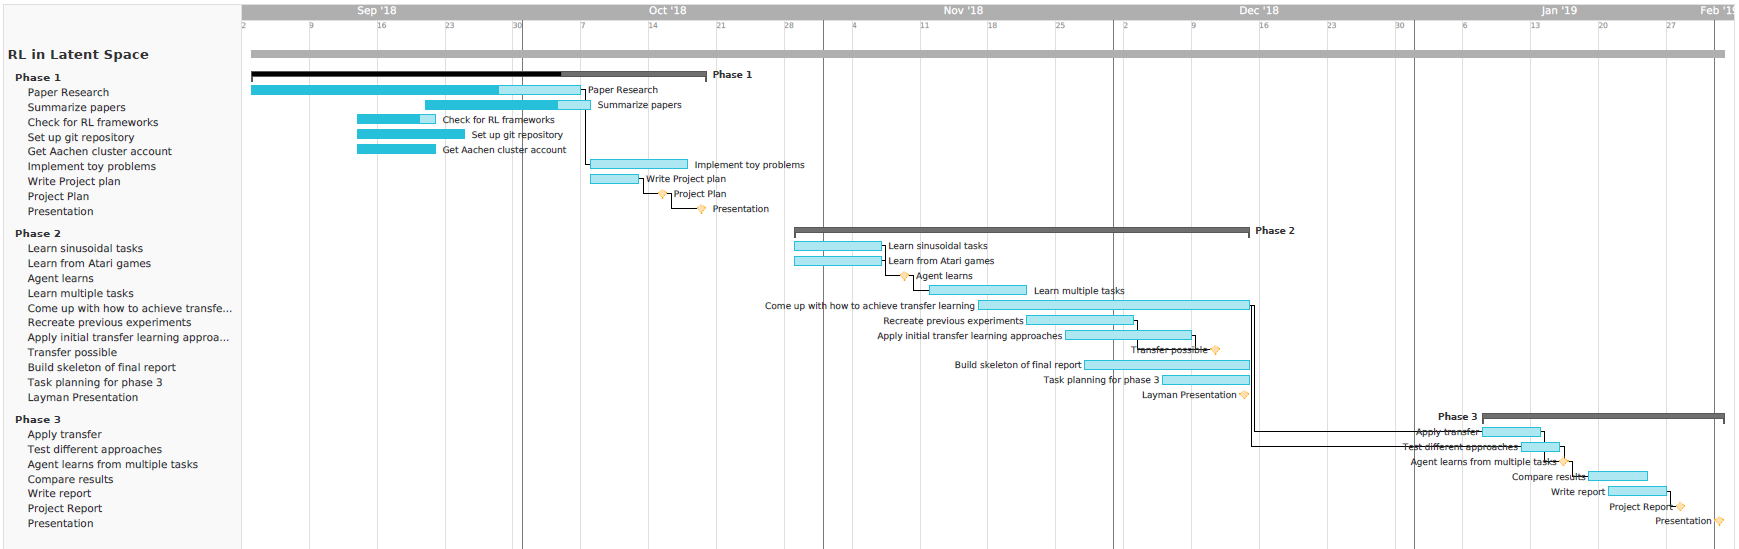
\includegraphics[scale=0.35]{ganttchart}

